\documentclass[format=acmtog]{acmart}

\title{Visualizing EEG signals}

\author{André Furlan}

\affiliation{
	\institution{UNESP - Universidade Estadual Paulista Júlio de Mesquita Filho}
	\city{São José do Rio Preto}
	\state{André Furlan}
	\country{Brazil}
}
\email{ensismoebius@gmail.com}

\begin{document}
	
	\begin{abstract}
		Electroencephalogram (EEG) data has inherent complexity, including a large volume, diverse frequencies (e.g., alpha, beta, theta, sigma), and numerous emitting sources (neurons). Additionally, potential electromagnetic interferences from external sources pose challenges during EEG analysis. This work aims to propose effective visualization techniques for EEG data, drawing insights from recent research on EEG visualization. The goal is to create informative visualizations that aid in EEG research by showing detailed representations of the data without the use of misleading gradients. The visualization will include interactive features for subject and stimulus selection, providing a comprehensive understanding of EEG signals with high-contrast color schemes to enhance perceptual clarity.
	\end{abstract}
	
	\maketitle
	
	\section{Introduction}
		\par Electroencephalogram (EEG) data is widely used in neuroscience research to study brain activity. EEG records electrical signals generated by brain neurons and reflects cognitive processes, making it a valuable tool in various applications, including Brain-Computer Interfaces (BCI) and clinical diagnosis of neurological disorders \cite{8937083}. Analyzing EEG data, however, poses challenges due to its complexity, such as a vast number of emitting sources (neurons) and potential electromagnetic interferences from external sources like cell phones, electric motors, and magnetic fields from wires \cite{8937083}. To facilitate EEG data interpretation and visualization, it is crucial to develop effective and efficient visualization techniques that allow researchers to gain valuable insights from the data. This paper proposes a novel visualization method for EEG data, combining line graphs and energy visualizations with a display of the electrode positions in the 10-20 system \cite{sistema10-20}. The proposed visualization will be interactive, allowing users to select subjects and stimuli and explore specific signal details. The goal is to provide researchers with an informative and comprehensive view of EEG data to support their investigations.
	
	\section{Data Acquisition}
	\par To demonstrate the proposed visualization technique, EEG data will be acquired from an existing dataset. The chosen dataset is the "Open access database of EEG signals recorded during imagined speech" \cite{10.1117/12.2255697}. This dataset contains EEG recordings during the imagined pronunciation of vowels and commands, as well as EEG and audio recordings during the actual pronunciation. The dataset includes recordings from 15 Argentinian volunteers between the ages of 24 and 28, with an equal representation of males and females \cite{10.1117/12.2255697}. The data aims to enable accessibility to EEG records during imagined speech for future research on Brain-Computer Interfaces (BCI) that classify words based on their imagination. Although this dataset serves as the initial data source for the proposed visualization, future research intends to develop a custom EEG database in collaboration with local health institutions.
	
	\section{Database Structure}
	The EEG dataset is organized to facilitate data manipulation and analysis. Each row in the dataset corresponds to a subject, and the data is arranged as follows: EEG signals from different electrodes, modalities (imagined or pronounced), and stimulus codes representing different categories of stimuli (e.g., letters and commands). The modalities distinguish between imagined and pronounced speech, while the stimulus codes identify specific categories of stimuli. Figure \ref{fig:visu04} shows a sample of the initial rows in the database, and Figure \ref{fig:visu05} displays the last rows.
	
	\begin{figure}
		\centering
		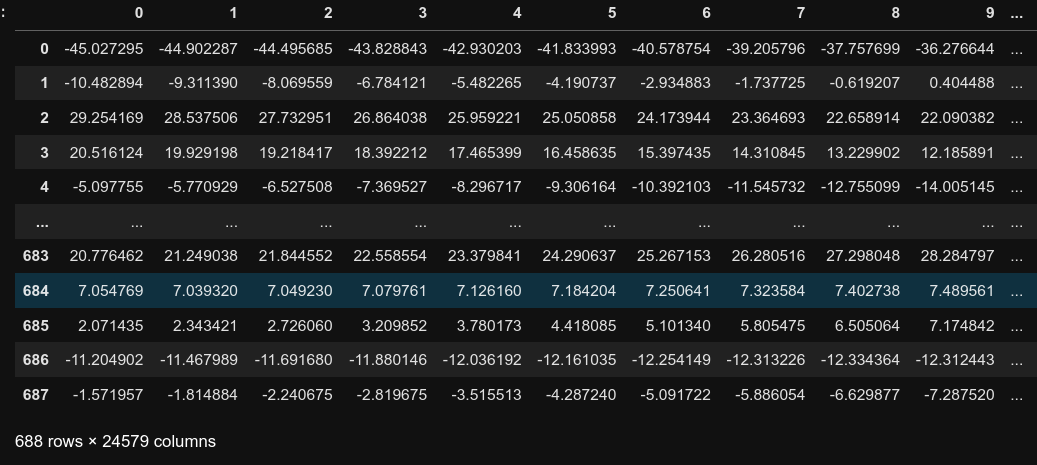
\includegraphics[width=\linewidth]{../presentation/images/visu04}
		\caption{Sample of initial rows in the EEG database}
		\label{fig:visu04}
	\end{figure}
	
	\begin{figure}
		\centering
		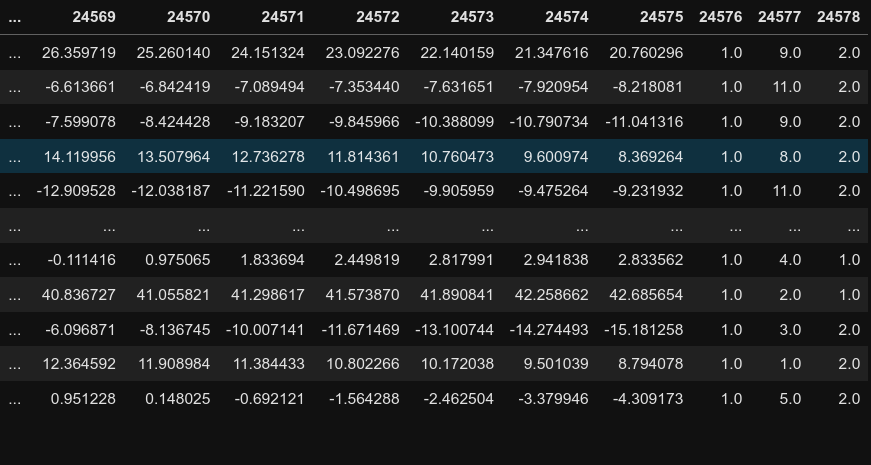
\includegraphics[width=.9\linewidth]{../presentation/images/visu05}
		\caption{Sample of last rows in the EEG database}
		\label{fig:visu05}
	\end{figure}
	
	\section{Pre-processing}
	To facilitate data manipulation and visualization, pre-processing techniques are applied to the EEG data. The data is grouped and organized to ensure seamless interactions and efficient representation. Figure \ref{fig:visu06} demonstrates the pre-processed and grouped data, ready for visualization.
	
	\begin{figure}
		\centering
		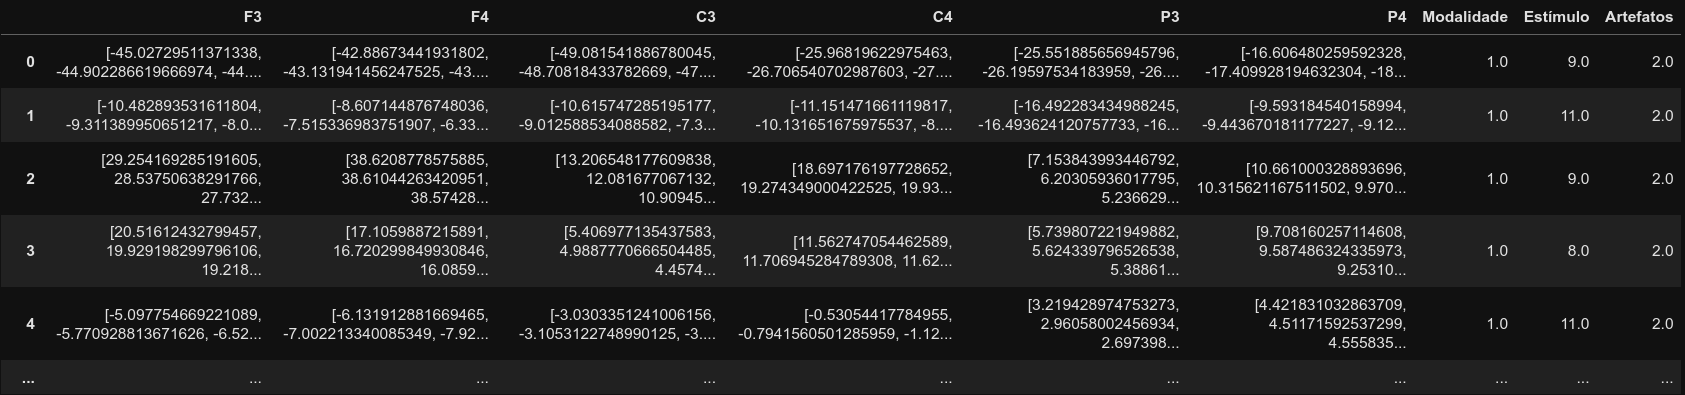
\includegraphics[width=\linewidth]{../presentation/images/visu06}
		\caption{Pre-processed and grouped EEG data}
		\label{fig:visu06}
	\end{figure}
	
	\section{Case Studies}
	The proposed visualization method will be evaluated through case studies using real EEG data. The case studies will focus on different subjects and stimuli to demonstrate the effectiveness and utility of the proposed visualization in various scenarios.
	
	\section{Visualization Inspired by EPviz \cite{currey2023epviz}}
	The proposed visualization method draws inspiration from EPviz, which effectively uses line graphs to visualize EEG data \cite{currey2023epviz}. EPviz visualizes EEG signals captured by all electrodes, providing a general overview of the data. However, the visualization lacks detailed views, which may limit the ability to discern specific patterns and features.
	
	\begin{figure}
		\centering
		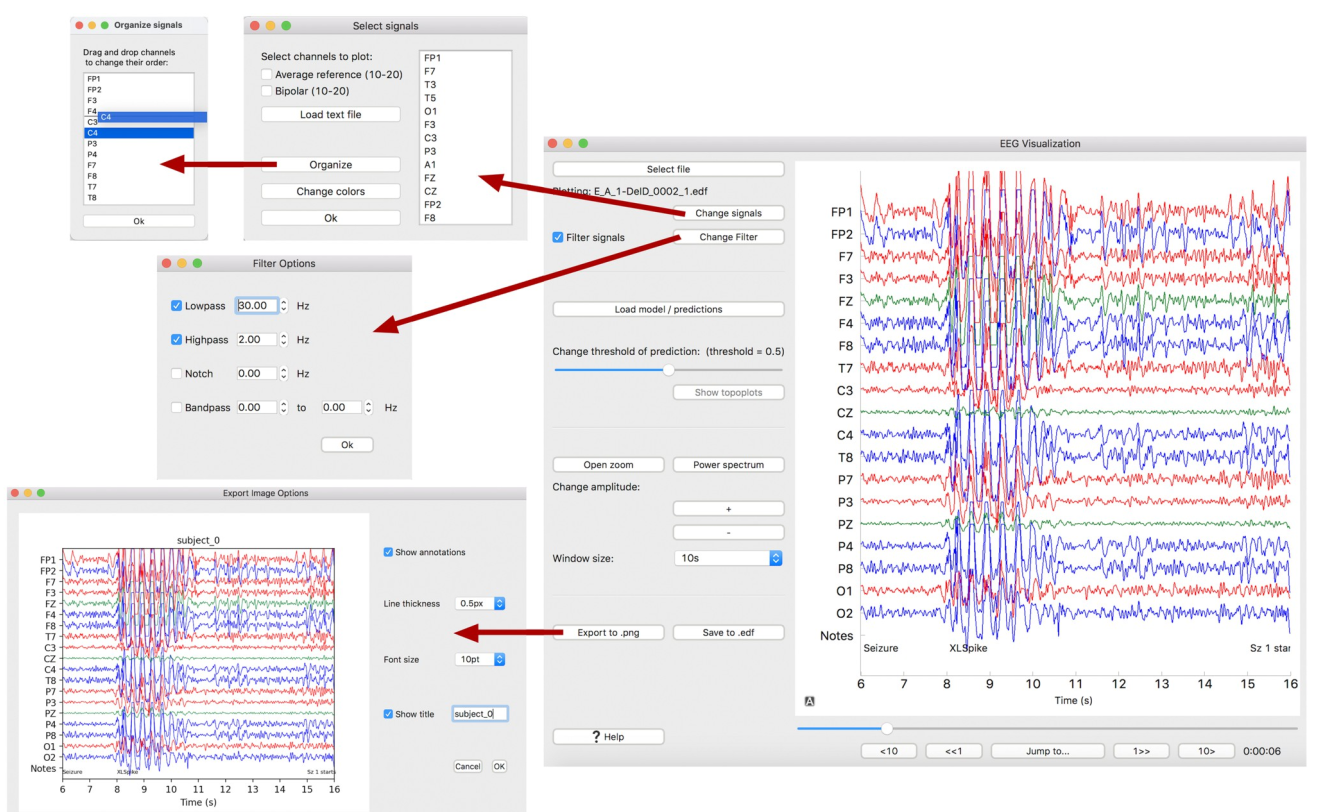
\includegraphics[width=\linewidth]{../presentation/images/epviz00}
		\caption{EPviz - Line graph visualization}
		\label{fig:epviz00}
	\end{figure}
	
	\section{Visualization Inspired by \cite{9098189}}
	Another relevant methodology uses topological color maps to indicate signal energy at each sensor, offering insights into brain activity \cite{9098189}. The visualization in Figure \ref{fig:visu01} provides an informative representation of regions with intense brain activity during the corresponding time period. However, the interpolation of measured values may lead to potential misinterpretations of signal intensities according to gradients.
	
	\begin{figure}
		\centering
		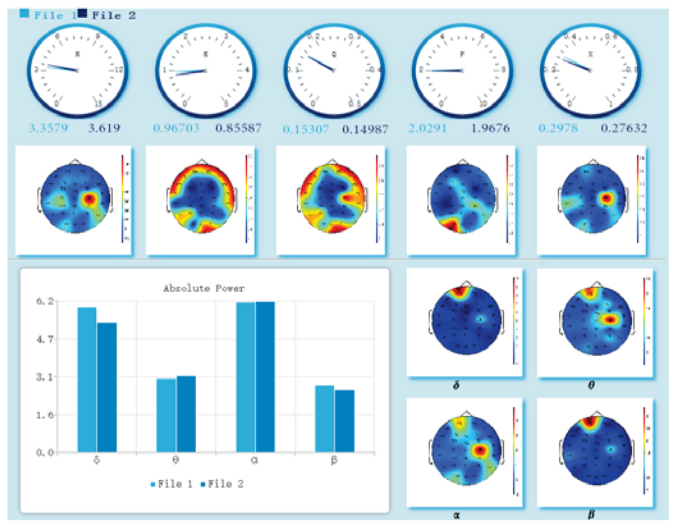
\includegraphics[width=\linewidth]{../presentation/images/visu01}
		\caption{Topological visualization}
		\label{fig:visu01}
	\end{figure}
	
	\section{Visualization Inspired by \cite{8937083}}
	This methodology simplifies the visualization to display brain activity at four different moments \cite{8937083}. However, similar to the previous visualization, the gradient issue persists, potentially leading to incorrect interpretations.
	
	\begin{figure}
		\centering
		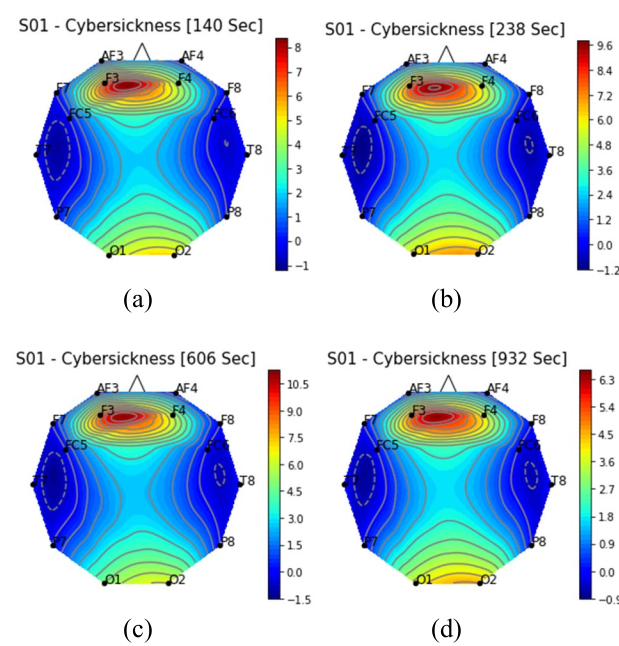
\includegraphics[width=\linewidth]{../presentation/images/visu02}
		\caption{Topological visualization}
		\label{fig:visu02}
	\end{figure}
	
	\section{Proposal}
	The proposed visualization method aims to overcome the limitations of existing techniques. It includes line graphs and energy visualizations combined with a non-gradient representation of electrode positions in the 10-20 system. The interactive features allow users to select subjects and stimuli, explore specific signal details, view the signal's origin, and amplify the displayed curves. Additionally, the visualization will include a bar showing the total energy of the displayed signal interval. The use of high-contrast colors will aid in perceptual differentiation. Figures \ref{fig:g3714} and \ref{fig:g3762} illustrate the general and specific views of the proposed visualization.
	
	\begin{figure}
		\centering
		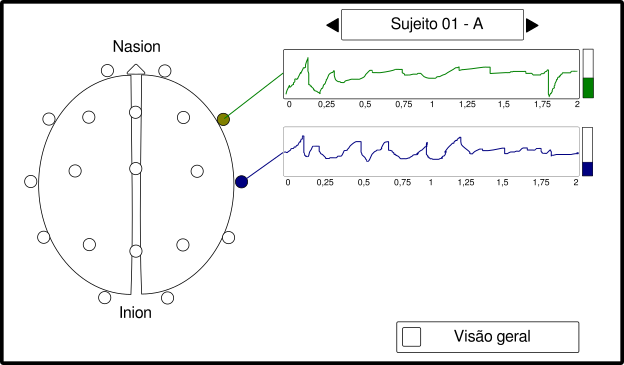
\includegraphics[width=\linewidth]{../presentation/images/g3714}
		\caption{General view of the proposed visualization}
		\label{fig:g3714}
	\end{figure}
	
	\begin{figure}
		\centering
		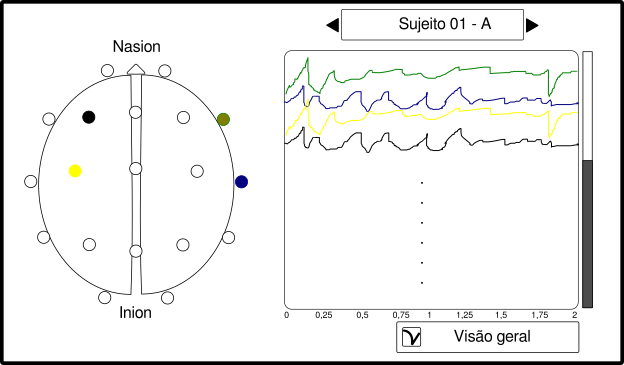
\includegraphics[width=\linewidth]{../presentation/images/g3762}
		\caption{Specific view of the proposed visualization}
		\label{fig:g3762}
	\end{figure}
	
	\section{Future Work}
	As the research progresses, the proposed visualization will be further developed to display the hierarchical decomposition of captured waves into their respective components ($\alpha$, $\beta$, $\theta$, $\sigma$). Additionally, the visualization will show the categories and classes to which each signal belongs.
	
	\section{Code Repository}
	To access the source code, please visit: \href{https://github.com/ensismoebius/VisualizacaoDeInformacao}{https://github.com/ensismoebius/VisualizacaoDeInformacao}
	
	\section{Conclusion}
	This work proposes a novel visualization method for EEG data, incorporating line graphs and energy visualizations with a non-gradient representation of electrode positions in the 10-20 system. The proposed visualization aims to facilitate EEG data analysis and interpretation by offering interactive features for subject and stimulus selection, as well as specific signal exploration. High-contrast colors will be employed to enhance perceptual clarity. Future research will extend the proposed visualization to include hierarchical representations of signal components and their associated categories and classes.
	
	\begin{acks}
		The author would like to thank the Universidade Estadual Paulista Júlio de Mesquita Filho for its support and resources during this research.
	\end{acks}
	
	\section{References}
	\bibliographystyle{ACM-Reference-Format}
	\bibliography{../presentation/bibliography.bib}
	
\end{document}
